%%%%%%%%%%%%%%%%%%%%%%%%%%%%%%%%%%%%%%%%%%%%%%%%%%%%%%%%%%%%%%%%%%%%%%%%%%
%%LaTeX template for papers && theses									%%
%%Done by the incredible ||Z01db3rg||									%%
%%Under the do what ever you want license								%%
%%%%%%%%%%%%%%%%%%%%%%%%%%%%%%%%%%%%%%%%%%%%%%%%%%%%%%%%%%%%%%%%%%%%%%%%%% 

%start preamble
\documentclass[paper=a4,fontsize=11pt]{scrartcl}%kind of doc, font size, paper size
\usepackage[ngerman]{babel}%for special german letters etc			
%\usepackage{t1enc} obsolete, but some day we go back in time and could use this again
\usepackage[T1]{fontenc}%same as t1enc but better						
\usepackage[utf8]{inputenc}%utf-8 encoding, other systems could use others encoding
%\usepackage[latin9]{inputenc}			
\usepackage{amsmath}%get math done
\usepackage{amsthm}%get theorems and proofs done
\usepackage{graphicx}%get pictures & graphics done
\graphicspath{{pictures/}}%folder to stash all kind of pictures etc
\usepackage{amssymb}%symbolics for math
\usepackage{amsfonts}%extra fonts
\usepackage []{natbib}%citation style
\usepackage{caption}%captions under everything
\usepackage{listings}
\usepackage[titletoc]{appendix}
\numberwithin{equation}{section} 
\usepackage[printonlyused,withpage]{acronym}%how to handle acronyms
\usepackage{float}%for garphics and how to let them floating around in the doc
\usepackage{cclicenses}%license!
\usepackage{xcolor}%nicer colors, here used for links
\usepackage{wrapfig}%making graphics floated by text and not done by minipage
\usepackage{dsfont}
\usepackage{stmaryrd}
\usepackage{geometry}
\usepackage{hyperref}
\usepackage{fancyhdr}
\usepackage{menukeys}
\usepackage{multicol}

%settings colors for links
\hypersetup{
    colorlinks,
    linkcolor={blue!50!black},
    citecolor={blue},
    urlcolor={blue!80!black}
}

\definecolor{pblue}{rgb}{0.13,0.13,1}
\definecolor{pgreen}{rgb}{0,0.5,0}
\definecolor{pred}{rgb}{0.9,0,0}
\definecolor{pgrey}{rgb}{0.46,0.45,0.48}

\pagestyle{fancy}
\lhead{Benjamin Tröster\\Netzwerke Übung (WiSe2018/19)}
\rhead{FB 4 -- Angewandte Informatik\\ HTW-Berlin}
\lfoot{Übungsblatt 04 -- Backbone Routing}
\cfoot{}
\fancyfoot[R]{\thepage}
\renewcommand{\headrulewidth}{0.4pt}
\renewcommand{\footrulewidth}{0.4pt}

\lstdefinestyle{Bash}{
  language=bash,
  showstringspaces=false,
  basicstyle=\small\sffamily,
  numbers=left,
  numberstyle=\tiny,
  numbersep=5pt,
  frame=trlb,
  columns=fullflexible,
  backgroundcolor=\color{gray!20},
  linewidth=0.9\linewidth,
  %xleftmargin=0.5\linewidth
}

\newlength\labelwd
\settowidth\labelwd{\bfseries viii.)}
\usepackage{tasks}
\settasks{counter-format =tsk[a].), label-format=\bfseries, label-offset=3em, label-align=right, label-width
=\labelwd, before-skip =\smallskipamount, after-item-skip=0pt}
\usepackage[inline]{enumitem}
\setlist[enumerate]{% (
labelindent = 0pt, leftmargin=*, itemsep=12pt, label={\textbf{\arabic*.)}}}

\pdfpkresolution=2400%higher resolution

%%here begins the actual document%%
\newcommand{\horrule}[1]{\rule{\linewidth}{#1}} % Create horizontal rule command with 1 argument of height

\DeclareMathOperator{\id}{id}

\begin{document}
\begin{center}\Large{\textbf{Aufgabe A -- Einrichten eines komplexen Netzwerkes mithilfe von Linux-Routern}}\end{center}\vskip0.25in
\textbf{Hilfreiche Programme:}
\begin{multicols}{3}
\begin{itemize}
	\item ifconfig, ip addr
	\item ip link
	\item route/ip route
	\item sysctl
	\item netstat, ss
	\item ping
\end{itemize}
\end{multicols}
Wir erweitern nun das vorhandene Netzwerk dergestalt, dass ein weiterer Rechner aus jeder Reihe zum Router umgebaut wird. Wenn genug Raspberry Pis vorhanden sind, kann auch ein zusätzlicher Raspberry Pi an den Switch angeschlossen werden. Der neue Router soll alle Pakete, die an Rechner außerhalb des eigenen Netzes gerichtet sind, in die anderen Reihen weiterleiten können. Somit können Sie dann jeden beliebigen Raspberry Pi im Labor anpingen. Die Router sorgen dafür, dass alle Pakete über das \glqq Backbone\grqq\ zu ihrem Ziel geleitet werden. Im wesentlichen soll das Netzwerk Abbildung \ref{backbone} entsprechen. 
\begin{figure}[H]
	\center
	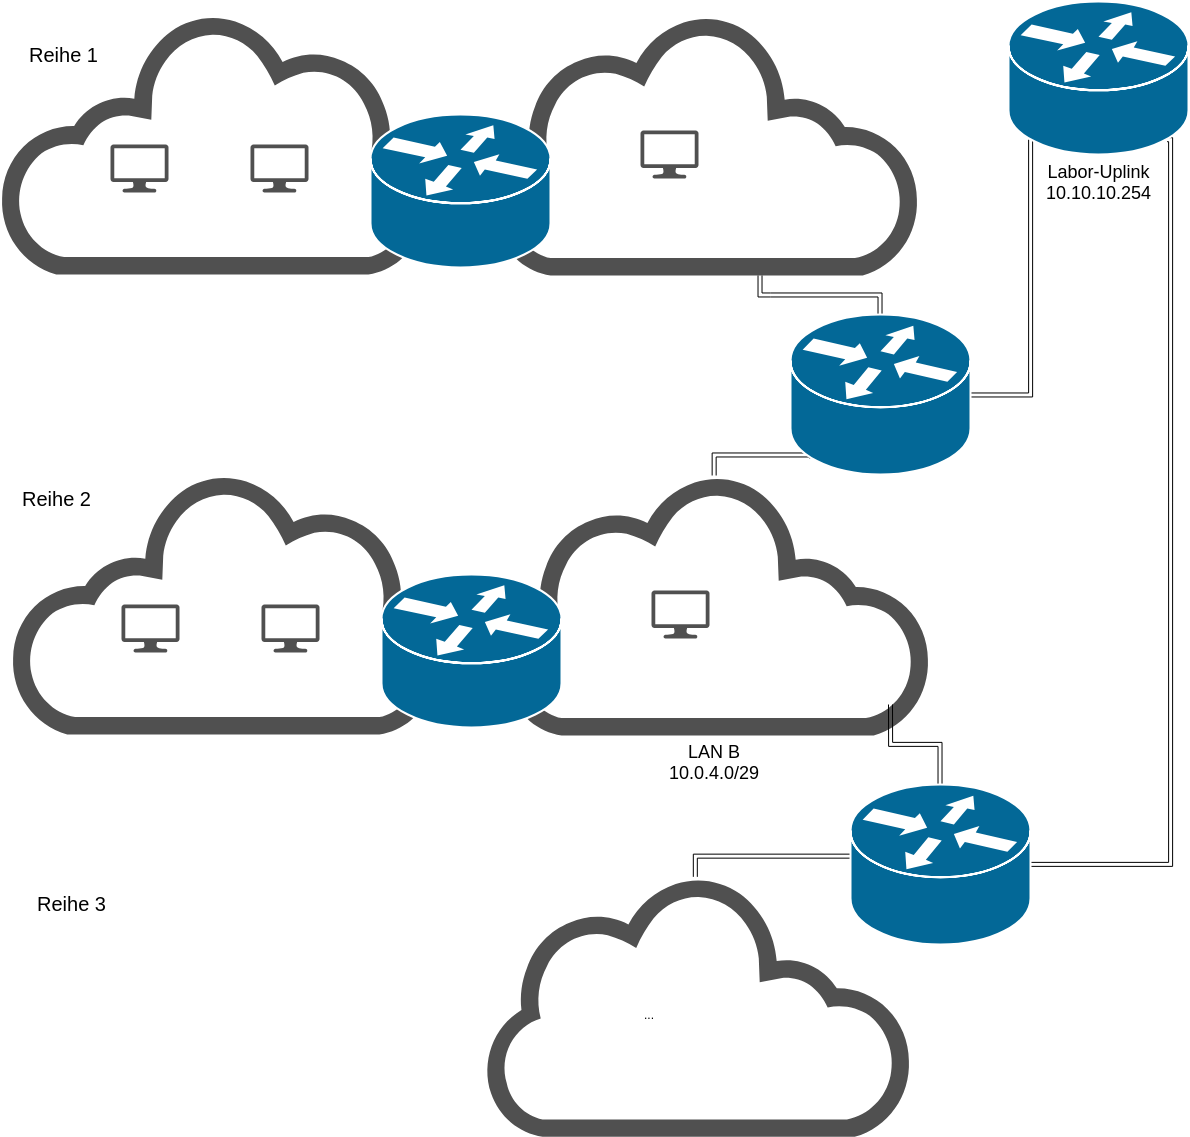
\includegraphics[scale=0.25]{backbone}
	\caption{Backbone-Netzwerk}
	\label{backbone}
\end{figure}
\begin{table}[H]
\caption{Adressschema für das Labor}
\label{adress_scheme}
\centering
\begin{tabular}{|c|c|}\hline
 & \textbf{IP  || IP-Range} \\ \hline
 $LAN_{A|B}$ & 10.0.$X_{\alpha|\beta}$.Y/Size \\ \hline
 Backbone & 10.10.10.100 + $\rho$ \\ \hline
 Labornetz & 10.0.0.0/8 \\ \hline
 Uplink & 10.10.10.254 \\ \hline
 DNS & 10.10.10.254 \\ \hline
\end{tabular}
\end{table} 
\vskip0.05in ~\\
\textbf{Achtung:} Da es in dem Backbone-Netz fünf gleichwertige Router gibt, können Sie hier nicht mit \glqq Default-Routes\grqq\ arbeiten! Sie müssen auf den Backbone-Rechnern nun mehrere explizite Routen mit einem Zielnetzwerk und zugehöriger Subnetzmaske eintragen.
\begin{enumerate}
	\item Schalten Sie zunächst wieder das DHCP aus! Vergewissern Sie sich, dass alle vorherigen IP-Adressen, Routen etc. gelöscht sind.
	\item Aufsetzen des Backbones:

\begin{tasks}(1)
	\task Wählen Sie einen Rechner aus Ihrer Reihe der noch nicht als Router fungiert. Geben Sie diesem Router eine zweite IP-Adresse 10.10.10.X, wobei $X=100 + \rho$ ist und $\rho$ Ihrer Reihe entspricht.\\
	\task Aktivieren Sie auf dem Backbone ebenfalls das Routing und tragen Sie alle Routen zu den anderen Reihen ein.
	\task Prüfen Sie mit \emph{ping}, ob Sie verschiedene Rechner innerhalb, sowie außerhalb Ihres Netzwerkes erreichen können -- bei welchen Rechner(n) klappt es und bei welchen nicht?
	\task Überprüfen Sie die Routen Ihrer Hosts! Haben die einfachen Hosts entsprechende Default-Routen? Hat Ihr Router eine Default-Route? Setzen Sie die Routen entsprechend, sodass im Anschluss alle Hosts sich untereinander erreichen können, als auch den Router und den Backbone-Router.
	\task Was müssen Sie jetzt noch an der Konfiguration einer oder aller anderen Rechner Ihrer Reihe anpassen, damit sich wirklich alle Rechner anpingen können.
	\task Befragen Sie als Hilfestellung den aktuellen Routing-Table Ihres Betriebssystems. Sie könne hierfür die Tools \emph{ip route, route, netstat -r} nutzen.
	\task Prüfen Sie mit \emph{ping} ob Sie jetzt wirklich alle Rechner erreichen können.
	\task Prüfen Sie mit \emph{Wireshark} auf dem neuen Backbone-Router, ob auch alle Pakete wirklich über diesen Rechner geleitet werden. Sie sollen ausschließen könne, dass irgendein Rechner eine \glqq Abkürzung\grqq\ nimmt.
	\task Sie können wie in der vorigen Übung einen kleinen Chatserver mit Netcat betreiben, um sich zu vergewissern, dass Ihr Netzwerk funktioniert.
\end{tasks}
\end{enumerate}

\begin{center}\Large{\textbf{Aufgabe B -- Einrichtung des Uplinks}}\end{center}\vskip0.25in
Seitdem Sie den DHCP-Dienst auf den Raspberry Pis ausgeschaltet haben, haben Sie keinen Uplink ins Internet mehr. Das soll sich mit dieser Aufgabe ändern.
\begin{enumerate}
	\item Um den Raspberry Pis eine Möglichkeit zu geben sich mit dem Internet zu verbinden, soll ein Uplink eingerichtet werden. Das heißt: Ihr konfigurierter Backbone-Router soll dafür sorgen, dass sie beispielsweise die Webseite der FU-Berlin anpingen können (die HTW-Berlin unterdrückt \emph{ICMP} aus nicht einsehbaren Gründen).
\begin{tasks}
  \task Erweitern Sie den Backbone-Router, sodass dieser den Uplink im Labor nutzen kann. Der Uplink ist auf dem Server im Dell-Rack untergebracht und besitzt die IP-Adresse: 10.10.10.254. Wie Sie bereits vermuten werden, muss Ihr Router nun die Pakete in dieses Netz bzw. an diesen Server weiterleiten können. Konfigurieren Sie entsprechend Ihren Router zunächst mit den Ihnen bekannten Tools \glqq on the fly \grqq.
  \task Welche Art Route müssen Sie auf dieses Gateway konfigurieren? \textbf{Hinweis:} Alle Pakete, die nicht an die Netzwerke des Labors adressiert sind, sollten dieses Gateway passieren.
  \task Befragen Sie als Hilfestellung den aktuellen Routing-Table Ihres Betriebssystems. Sie könne hierfür die Tools \emph{ip route, route, netstat -r} nutzen.
  \task Nachdem die Wahl der Routen und somit das Routing erledigt ist, müssen Sie sich um das NAT kümmern. Da im Labor nur private IPv4-Adressen genutzt werden, müssen diese entsprechend übersetzt werden. Im DHCP-Modus erledigt dies direkt der Uplink.\\
  Da Sie nun selbst für Ihre Infrastruktur verantwortlich sind, müssen Sie dies übernehmen. Mithilfe von \emph{iptables} kann ein Masquerading vorgenommen werden (SNAT). Das Masquerading übernimmt die Aufgabe, die Pakete Ihrer internen Netzwerke zu übersetzen und die Replies entsprechend wieder in das Netzwerk zu schicken.\\
  Setzen Sie auf dem Backbones die Network-Address-Translation mithilfe von \emph{iptables} um.
  \task Da auf dem Uplink bereits ein DNS-Server arbeitet, müssen Sie sich keine Sorgen hierüber machen. Sie sollten nun sowohl IP-Adressen als auch Host-Names adressieren können.
  \task Versuchen Sie die Website der Freien Universität Berlin anzupingen.
\end{tasks}
\end{enumerate}

\begin{center}\Large{\textbf{Aufgabe C -- IPv6}}\end{center}\vskip0.25in
Da \emph{IPv4} ein etwas betagteres Protokoll ist und Sie Fit für die Zukunft sein sollten, sollen Sie abschließend Ihr Netzwerk mittels \emph{IPv6} umsetzen. Da \emph{IPv6} eine wesentlich größere IP-Range besitzt ist in der Nachfolgenden Tabelle ein mögliches Adressschema aufgezeigt. Auch hier gilt: \emph{IPv6} hat mehr Adressen, dies sollte Sie jedoch nicht dazu verleiten, verschwenderisch damit umzugehen!
\begin{table}[H]
\centering
\begin{tabular}{ll}
 Prefix/L & fd  \\
 Global ID & 0da5a0170a \\
 Subnet ID &  5fd7\\
 Combined/CID & fd0d:a5a0:170a:5fd7::/64 \\
 IPv6 addresses & fd0d:a5a0:170a:5fd7:xxxx:xxxx:xxxx:xxxx 
\end{tabular}
\end{table}
Sie sollen im Folgenden ein statisches \emph{IPv6}-Netzwerk umsetzen. Ein Routing außerhalb unseres Labornetzwerkes ist leider nicht möglich, da die HTW Berlin momentan kein \emph{IPv6} einsetzt.
\begin{enumerate}
	\item Adaptieren Sie Ihren Netzwerkaufbau von \emph{IPv4} auf \emph{IPv6}. D.h. der grundsätzliche Aufbau des Netzwerkes soll nicht verändert werden, nur das Netwrok-Layer-Protokoll soll sich ändern!
	\item Vergeben Sie in Ihrem Netzwerk entsprechende Adressen. Vergessen Sie nicht entsprechende Adressen für die Router zu setzen.
	\item Setzen Sie Routen, sodass die Raspberry Pis sich über ihre LANs hinweg erreichen.
	\item Testen Sie Ihre Netzwerke mit \emph{ping}.
\end{enumerate}

\begin{center}\Large{\textbf{System Reset}}\end{center}\vskip0.25in
\begin{enumerate}
	\item \textbf{Sofern Sie keine eigene SD-Karte nutzen:} Setzen Sie die Einstellungen des Raspberry Pis bzw. des Betriebssystems zurück die Sie vorgenommen haben! D.h. setzen Sie das Betriebssystem auf den \emph{dhcpcd} zurück, nehmen Sie alle vorgenommen Änderungen zurück. Haken Sie zumindest folgende Liste ab:
\begin{itemize}
	\item Eigene IP-Config zurücksetzen:
	\begin{itemize}
		\item \path{/etc/network/interfaces}
		\item Bash-Script: \emph{reset\_network\_config.sh}
	\end{itemize}
	\item Routing/Forwarding:
	\begin{itemize}
		\item Keine persistenten Routen vorhanden?
		\item Forwarding deaktiviert? 
		\item \path{/etc/systctl.conf}
		\item \path{/proc/sys/net/ipv4/ip_forward}
	\end{itemize}
	\item DNS
	\begin{itemize}
		\item DNS Einträge verändert?
		\item \path{/etc/resolv.conf}
		\item \emph{reset\_hosts.sh}
	\end{itemize}
	\item DHCPcd:
	\begin{itemize}
		\item \emph{sudo systemctl enable dhcpcd}
		\item \emph{nw\_default.sh}
	\end{itemize}
\end{itemize}
\end{enumerate}
\end{document}